\begin{frame}[allowframebreaks]{DreamFusion: Text-to-3D Generation}
    \large How can you use a pretrained text-image model to generate 3D objects?
    \begin{figure}
        \centering
        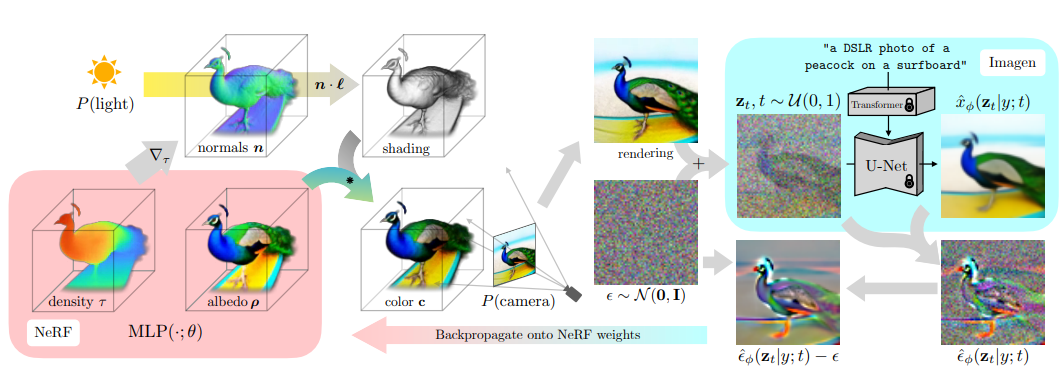
\includegraphics[width=1.05\linewidth,height=\textheight,keepaspectratio]{images/adv-img-gen/slide_151_1_img.png}
        \caption*{Poole, Ben, et al. "Dreamfusion: Text-to-3d using 2d diffusion." arXiv preprint arXiv:2209.14988 (2022).}
    \end{figure}

    \framebreak
    \large Start with a randomly initialized parameterized 3D representation (NeRF)
    \begin{figure}
        \centering
        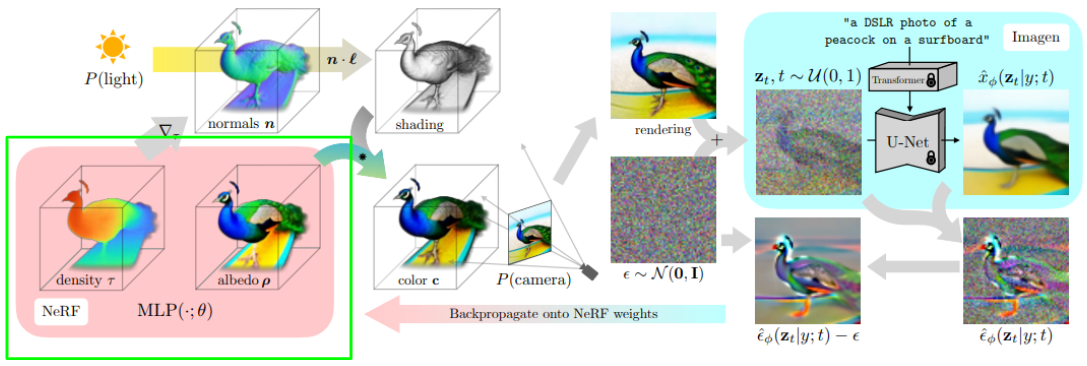
\includegraphics[width=1.05\linewidth,height=\textheight,keepaspectratio]{images/adv-img-gen/slide_152_1_img.png}
    \end{figure}

    \framebreak
    \large Randomly sample camera angle and lighting
    \begin{figure}
        \centering
        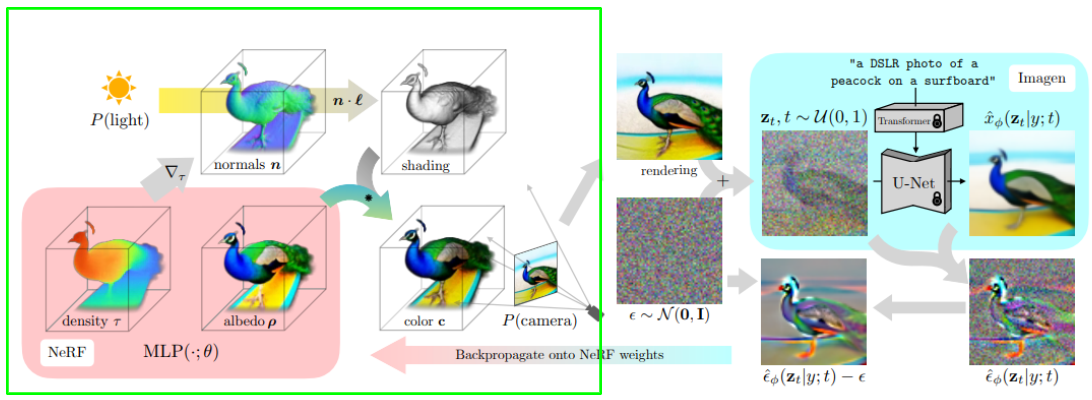
\includegraphics[width=1.05\linewidth,height=\textheight,keepaspectratio]{images/adv-img-gen/slide_153_1_img.png}
    \end{figure}

    \framebreak
    \large Render the image $(64 x 64)$
    \begin{figure}
        \centering
        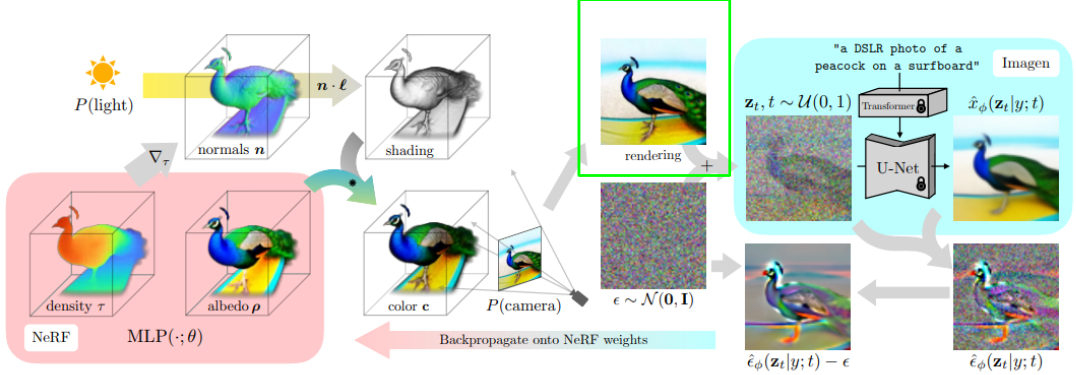
\includegraphics[width=1.05\linewidth,height=\textheight,keepaspectratio]{images/adv-img-gen/slide_154_1_img.png}
    \end{figure}

    \framebreak
    \large Noise the image and feed it through the diffusion loss to predict the noise
    \begin{figure}
        \centering
        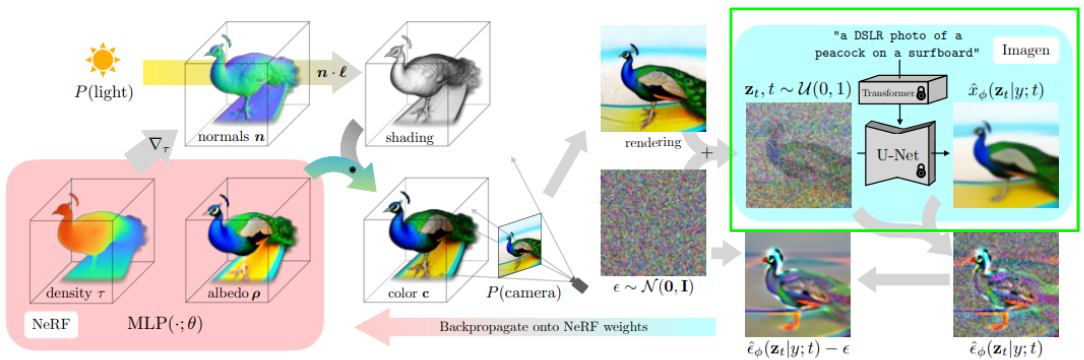
\includegraphics[width=1.05\linewidth,height=\textheight,keepaspectratio]{images/adv-img-gen/slide_155_1_img.png}
    \end{figure}

    \framebreak
    \large Compute the SDS loss and backpropagate
    \begin{figure}
        \centering
        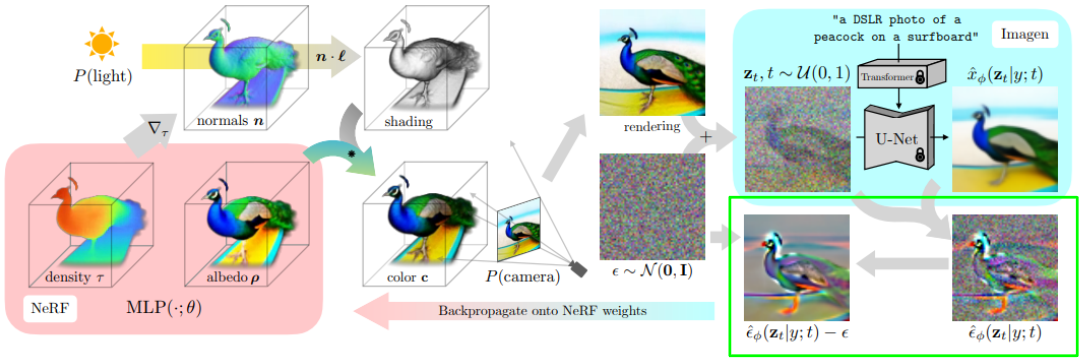
\includegraphics[width=1.05\linewidth,height=\textheight,keepaspectratio]{images/adv-img-gen/slide_156_1_img.png}
    \end{figure}

    \framebreak

    Intuitively, we want the NeRF parameters to produce images that minimize the diffusion loss
    \begin{figure}
        \centering
        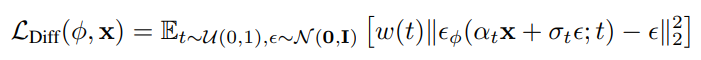
\includegraphics[width=0.85\linewidth,height=\textheight,keepaspectratio]{images/adv-img-gen/slide_157_1_img.png}
    \end{figure}\begin{figure}
        \centering
        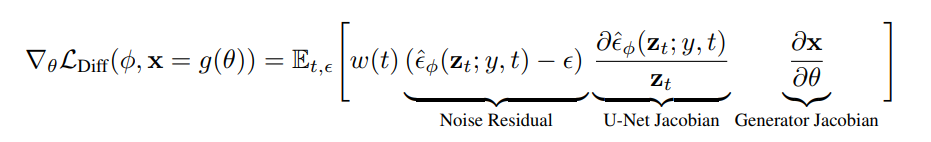
\includegraphics[width=1.05\linewidth,height=\textheight,keepaspectratio]{images/adv-img-gen/slide_157_2_img.png}
    \end{figure}
    But the objective is generally brittle / expensive (backprop through the UNet)

    \framebreak
    It works better to just remove the U-Net jacobian
    \begin{figure}
        \centering
        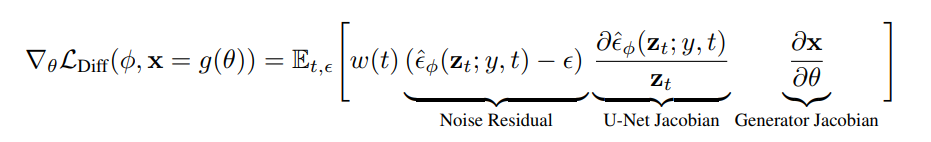
\includegraphics[width=1.05\linewidth,height=\textheight,keepaspectratio]{images/adv-img-gen/slide_158_1_img.png}
    \end{figure}\begin{figure}
        \centering
        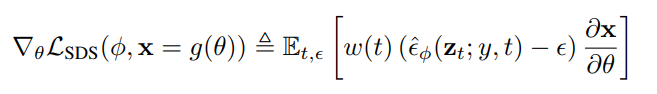
\includegraphics[width=1.05\linewidth,height=\textheight,keepaspectratio]{images/adv-img-gen/slide_158_2_img.png}
    \end{figure}
    There is a theoretical motivation (see Appendix in \href{https://arxiv.org/abs/2209.14988}{paper})

    \framebreak
    \begin{figure}
        \centering
        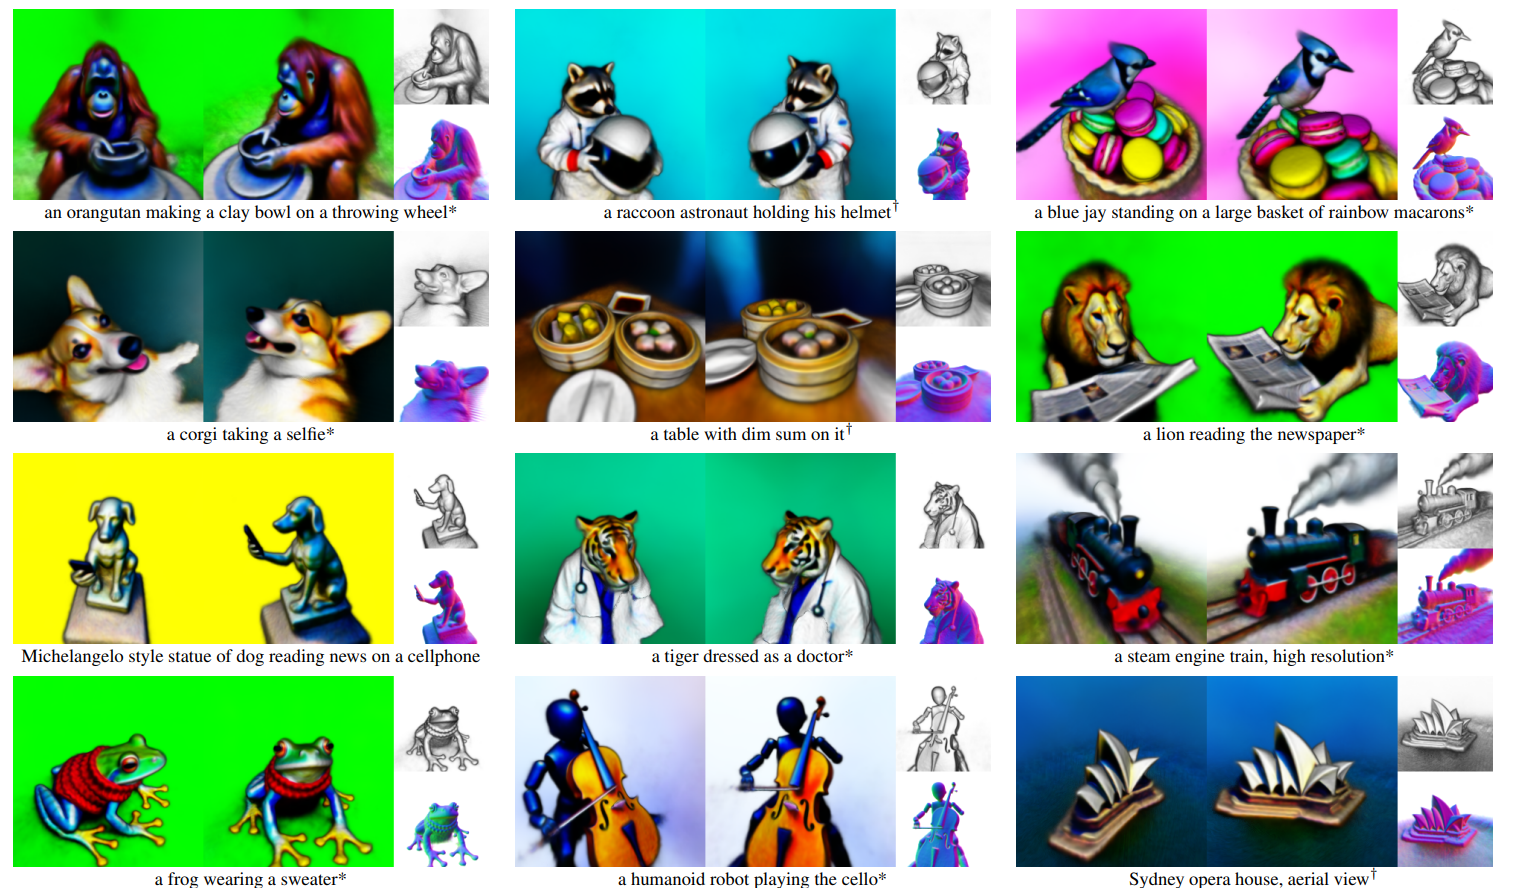
\includegraphics[width=1.05\linewidth,height=\textheight,keepaspectratio]{images/adv-img-gen/slide_159_1_img.png}
    \end{figure}
\end{frame}